%*******************************************************************************
%*********************************** First Chapter *****************************
%*******************************************************************************

\chapter{Tổng quan}  %Title of the First Chapter

\ifpdf
    \graphicspath{{Chapter1/Figs/Raster/}{Chapter1/Figs/PDF/}{Chapter1/Figs/}{}}
\else
    \graphicspath{{Chapter1/Figs/Vector/}{Chapter1/Figs/}}
\fi


%********************************** %First Section  **************************************
\section{Mở đầu} %Section - 1.1 
\subsection{Mục đích đề tài}
Trong cuộc sống bận rộn hiện nay, con người chúng ta hay có xu hướng bị xao nhãng và bỏ quên các thiết bị nhỏ. trong đó có thiết bị điện thoại di động và chùm chìa khóa là hai vật rất quan trọng và thường hay bỏ quên nhất. Và tìm kiếm chúng không hề dễ dàng, nhất là khi đang vội thì sẽ làm mọi thứ rối tung lên.

Từ điều đó đã thúc đẩy nhóm chúng tôi tìm cách giải quyết và nảy ra ý tưởng tạo ra sản phẩm móc khóa thông mình - Smart Keyring có chức năng kết nối với thiết bị di động sử dụng công nghệ BLE để giải quyết vấn đề trên dựa trên các tính năng của BLE.
\subsection{Giới thiệu về công nghê Bluetooth}
Ngày nay, xã hội phát triển mạnh mẽ, kỹ thuật ngày càng hiện đại nên nhu cầu về trao đổi thông tin, giải trí, nhu cầu về điều khiển thiết bị từ xa,…ngày càng cao. Và những hệ thống dây cáp phức tạp lại không thể đáp ứng tốt nhu cầu này, nhất là ở những khu vực chật hẹp, những nơi xa xôi, trên các phương tiện vận chuyển,…Vì thế công nghệ không dây đã ra đời và đang phát triển mạnh mẽ, tạo rất nhiều thuận lợi cho con người trong đời sống hằng ngày. Kỹ thuật không dây phục vụ rất nhiều nhu cầu khác nhau của con người, từ nhu cầu làm việc, học tập đến các nhu cầu giải trí như chơi game, xem phim, nghe nhạc, v.v…Với các nhu cầu đa dạng và phức tạp đó, kỹ thuật không dây đã đưa ra nhiều chuẩn với các đặc điểm kỹ thuật khác nhau để có thể phù hợp với từng nhu cầu, mục đích và khả năng của người sử dụng như IrDA, WLAN với chuẩn 802.11, ZigBee, OpenAir, UWB, Bluetooth,…

Mỗi chuẩn kỹ thuật đều có những ưu, khuyết điểm riêng của nó, và Bluetooth đang dần nổi lên là kỹ thuật không dây tầm ngắn có nhiều ưu điểm, rất thuận lợi cho những thiết bị di động. Với một tổ chức nghiên cứu đông đảo, hiện đại và số lượng nhà sản xuất hỗ trợ kỹ thuật Bluetooth vào sản phẩm của họ ngày càng tăng, Bluetooth đang dần lan rộng ra khắp thế giới, xâm nhập vào mọi lĩnh vực của thiết bị điện tử và trong tương lai mọi thiết bị điện tử đều có thể được hỗ trợ kỹ thuật này.

	\begin{table}[ht]
		\begin{tabular}{ |c|m{2cm}|m{2cm}|m{2cm}|m{2cm}| } 
			\hline
			& \textbf{Bluetooth} & \textbf{BLE} & \textbf{Wifi} & \textbf{Zigbee} \\ 
			\hline
			\textbf{Radio Frequency} &	2.4G &	2.4G &	2.4G &	2.4G \\ 
			\hline
			\textbf{Distance Range} &	10m	&>60m &	30m	& 10-100m \\ 
			\hline
			\textbf{Air Datarate} &	1-3Mbps &	1Mbps &	54Mbps &	250kbps \\
			\hline
			\textbf{Application Throughput} &	0.7-2.1Mbps &	305kbps &Depend &120kbps\\
			\hline
			\textbf{Security} &	64bit, 128bit &	128-bit & AES	SSID, WEP&	128-bit AES \\
			\hline
			\textbf{Power consumption}&	Low	&Very Low&	High&	Low \\
			\hline
			\textbf{Certification Body}&	Bluetooth SIG&	Bluetooth SIG&	IEEE802.11&	IEEE802.15.4 \\
			\hline
			\textbf{Network topology} &	Point-to-Point Scatternet&	Point-to-Point Star&	Point-to-Hub& 		Mesh, Ad-hoc\\
			\hline
		\end{tabular}
		\caption {Bảng so sánh các công nghệ truyền không dây}
		\label{table:1.1}
	\end{table}
\subsection{Mục tiêu - Phạm vi - Đối tượng nghiên cứu}

Xuất phát từ các lý do trình bày ở trên, chúng tôi đã thực hiện đề tài “Thiết kế sản phẩm móc khóa thông minh (Smart Keyring) dựa trên nền tảng công nghệ Bluetooth Low Energy (BLE)”. Mục tiêu của đề tài là:

- Tìm hiểu về công nghệ Bluetooth

- Kế thiết bị “Móc khóa thông minh - SmartKeyring” sử dụng công nghệ

Bluetooth và kết nối với ứng dụng Android trên điện thoại.

\nomenclature[z-cif]{$CIF$}{Cauchy's Integral Formula}                                % first letter Z is for Acronyms 
\nomenclature[a-F]{$F$}{complex function}                                                   % first letter A is for Roman symbols
\nomenclature[g-p]{$\pi$}{ $\simeq 3.14\ldots$}                                             % first letter G is for Greek Symbols
\nomenclature[g-i]{$\iota$}{unit imaginary number $\sqrt{-1}$}                      % first letter G is for Greek Symbols
\nomenclature[g-g]{$\gamma$}{a simply closed curve on a complex plane}  % first letter G is for Greek Symbols
\nomenclature[x-i]{$\oint_\gamma$}{integration around a curve $\gamma$} % first letter X is for Other Symbols
\nomenclature[r-j]{$j$}{superscript index}                                                       % first letter R is for superscripts
\nomenclature[s-0]{$0$}{subscript index}                                                        % first letter S is for subscripts


%********************************** %Second Section  *************************************
\section{Tổng quan về công nghệ Bluetooth} %Section - 1.2

\subsection{Khái niệm Bluetooth}
Bluetooth là công nghệ không dây cho phép các thiết bị điện, điện tử giao tiếp với nhau trong khoảng cách ngắn, bằng sóng vô tuyến qua băng tần chung ISM (Industrial, Scientific, Medical) trong dãy tầng 2.40- 2.48 GHz. Đây là dãy băng tầng không cần đăng ký được dành riêng để dùng cho các thiết bị không dây trong công nghiệp, khoa học, y tế.
	\begin{figure}[ht]
		\centering    
		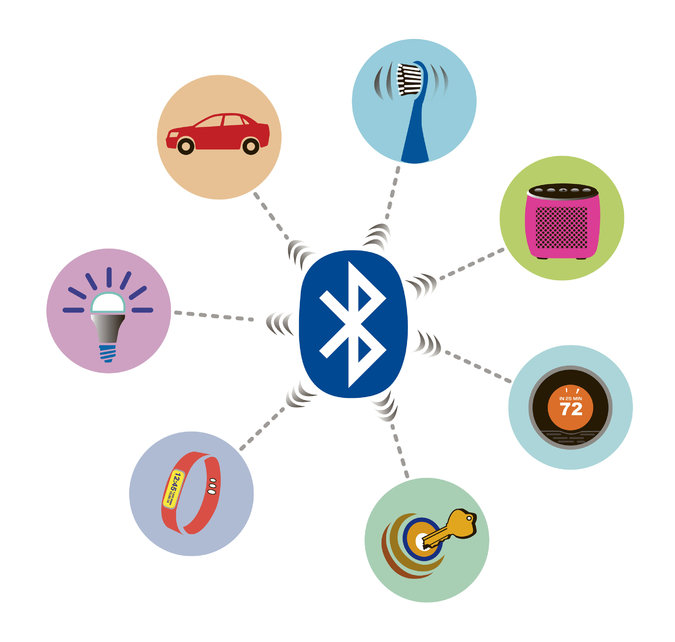
\includegraphics[width=0.7\textwidth]{btuse}
		\caption[Các ứng dụng Bluetooth]{Các ứng dụng Bluetooth}
		\label{fig:btuse}
	\end{figure}
	
Bluetooth được thiết kế nhằm mục đích thay thế dây cable giữa máy tính và các thiết bị truyền thông cá nhân, kết nối vô tuyến giữa các thiết bị điện tử lại với nhau một cách thuận lợi với giá thành rẻ. Khi được kích hoạt, Bluetooth có thể tự động định vị những thiết bị khác có chung công nghệ trong vùng xung quanh và bắt đầu kết nối với chúng. Nó được định hướng sử dụng cho việc truyền dữ liệu lẫn tiếng nói.

\subsection{Đặc điểm của Bluetooth}
- Tiêu thụ năng lượng thấp, cho phép ứng dụng được trong nhiều loại thiết bị, bao gồm cả các thiết bị cầm tay và điện thoại di động.

- Giá thành hạ (giá một chip Bluetooth đang giảm dần)

- Khoảng cách giao tiếp cho phép :

• Khoảng cách giữa hai thiết bị đầu cuối có thể lên đến 10m ngoài trời, và 5m

trong tòa nhà.

• Khoảng cách thiết bị đầu cuối và Access point có thể lên tới 100m ngoài trời và 30m trong tòa nhà.

- Bluetooth sử dụng băng tần không đăng ký 2.4Ghz trên dãy băng tần ISM. Tốc độ truyền dữ liệu có thể đạt tới mức tối đa 1Mbps (do sử dụng tần số cao) mà các thiết bị không cần phải thấy trực tiếp nhau (light-of- sight requirements)

- Dễ dàng trong việc phát triển ứng dụng: Bluetooth kết nối một ứng dụng này với một ứng dụng khác thông qua các chuẩn “Bluetooth profiles”, do đó có thể độc lập về phần cứng cũng như hệ điều hành sử dụng.

- Bluetooth được dùng trong giao tiếp dữ liệu tiếng nói: có 3 kênh để truyền tiếng nói, và 7 kênh để truyền dữ liệu trong một mạng cá nhân.

- An toàn và bảo mật: được tích hợp với sự xác nhận và mã hóa ( build in authentication and encryption)

- Tính tương thích cao, được nhiều nhà sản xuất phần cứng cũng như phần mềm hỗ trợ.

\subsection{Quá trình phát triển}
\label{history}
% TODO: nguồn wiki link chú thích bla bla bla
Đặc tả Bluetooth được phát triển đầu tiên bởi Ericsson (hiện nay là Sony Ericsson và Ericsson Mobile Platforms), và sau đó được chuẩn hoá bởi Bluetooth Special Interest Group (SIG). Chuẩn được phát hành vào ngày 20 tháng 5 năm 1999. Ngày nay được công nhận bởi hơn 1800 công ty trên toàn thế giới. Được thành lập đầu tiên bởi Sony Ericsson, IBM, Intel, Toshiba và Nokia, sau đó cùng có sự tham gia của nhiều công ty khác với tư cách cộng tác hay hỗ trợ. Bluetooth có chuẩn là IEEE 802.15.1.

\textbf{Các phiên bản Bluetooth:}

% TODO: nguồn thegioididong.com
1.    Bluetooth 1.0: Là phiên bản đầu tiên của chuẩn kết nối Bluetooth được đưa vào sử dụng với tốc độ truyền tải dữ liệu là 1Mbs, tuy nhiên thực tế tốc độ của phiên bản này chỉ đạt được mức 720kbs.

2.    Bluetooth 2.0 + ERD: Phiên bản nâng cấp sau Bluetooth 1.0 được nâng cấp tốc độ truyền tải lên 2.1 Mbs cùng với chế độ truyền tải mới ERD (enhanced data rate). Phiên bản 2.1 được nâng cấp về tốc độ truyền tải nhưng lại hạn chế trên thiết bị sử dụng do ERD chỉ là chế độ tùy chọn, một số nhà sản xuất đã không đưa chế độ này vào sản phẩm của mình để giảm chi phí sản xuất.

3.    Bluetooth 2.1+ ERD: Được nâng cấp từ Bluetooth 2.0 vào năm 2007 với thay đổi quan trọng như hiệu năng cao hơn, giảm điện năng tiêu thụ. Phiên bản này được sử dụng trên các thiết bị như điện thoại di độn, laptop, tai nghe ….. Tuy nhiên, Bluetooth 2.1 vẫn chưa cho người dùng truyền tải các tập tin có dung lượng lớn.

4.    Bluetooth 3.0 + HS: Năm 2009 buetooth 3.0 ra đời với thay đổi lớn về tốc độ truyền tải, đạt 24Mbps ở phiên bản này các thiết bị có thể tương tác dễ dàng với nhau hơn, có thể tự dò tìm các thiết bị ở gần.

5.    Bluetooth 4.0 - Bluetooth Low Energy: Là sự kết hợp của các đời Bluetooth trước đó với nhau. Bluetooth 4.0 đạt tốc độ truyền tải lên đến 25Mbps, dễ dàng ghép đôi các thiết bị với nhau, hiệu năng tiêu thụ thấp. Đây là chuẩn Bluetooth được sử dụng trên hầu hết các thiết bị hiện nay.

6.    Bluetooth 4.1 và 4.2: Là phiên bản ra đời đầu năm 2014 với nhiều cải tiến vượt bậc so với Bluetooth 4.0 như khả năng điều chống chồng chéo tín hiệu, kết nối thực sự thông minh và khả năng truyền dữ liệu độc lập mà không cần phụ thuôc vào trung tâm điều khiển. Phiên bản 4.2 được phát triển có khả năng truyền tải cao và bảo mật hơn, nhưng quan trọng hơn cả là cho phép các vi xử lý sử dụng chuẩn giao thức Ipv6 để truy cập trực tiếp vào internet.

7.	Bluetooth 5.0: theo dự kiến sẽ bắt đầu xuất hiện trên các thiết bị thương mại vào cuối 2016 nay hoặc đầu năm 2017 (Q1). Bluetooth 5.0 có tầm phủ sóng tăng lên gấp 4 lần so với Bluetooth 4.2 hiện nay, còn tốc độ truyền dữ liệu thì tăng lên cao nhất là 2 lần. Việc mở rộng khả năng phủ sóng của Bluetooth sẽ giúp các thiết bị Internet of Things sẽ có thể giao tiếp với nhau cũng như với trạm điều khiển một cách dễ dàng hơn, vượt qua bức tường của một căn nhà bình thường, trong khi lại tăng tốc thu thập và truyền dữ liệu. Chuẩn Bluetooth mới cũng sẽ giúp các beacon và giải pháp nhận diện địa điểm trở nên thông minh, chính xác và phản hồi nhanh hơn với sự hiện diện của người dùng.

% theo http://www.pcmag.com/news/345316/bluetooth-5-0-to-quadruple-range-double-speed
%********************************** % Third Section  *************************************
\section{Bluetooth Low Energy (BLE) }  %Section - 1.3 
\label{section1.3} %TODO ref htelectronic
Như đã được đề cập ở mục \ref{history}, BLE xuất hiện từ phiên bản 4.0, là một bước ngoặc lớn trong sự phát triển kết nối không dây. Các mạch BLE rất nhỏ cùng với công suất tiêu thụ hiệu năng cực thấp (khoảng vài chục uA khi hoạt động), nên hầu hết các thiết bị đều có thể tích hợp công nghệ này, từ các thiết bị nhỏ bé như tai nghe, chìa khóa.. cho tới các thiết bị lớn như tủ lạnh, tivi, xe máy... Nhờ đó, các thiết bị có thể trở nên "smart".
\subsection{Phân loại vai trò thiết bị BLE}
Có 4 loại thiết bị BLE (có thể gọi là chế độ hoạt động) đó là Peripheral, Central, Observer và Broadcaster và bình thường thì một thiết bị BLE chỉ hoạt động  trong một chế độ.

• \textbf{Central} là thiết bị sẽ chủ động yêu cầu kết nối đến các thiết bị BLE khác (thường là smartphone, tablet). Sau khi kết nối thì chúng ta lại gọi BLE Central là  BLE Master.

• \textbf{BLE Peripheral} là thiết bị chấp nhận yêu cầu kết nối (thường là đồ vật BLE). Tương tự, sau khi kết nối thì chúng ta gọi BLE Peripheral là BLE Slave.

• \textbf{BLE Observer} là BLE Central nhưng chỉ nhận dữ liệu nhận dạng của các thiết bị xung quanh nhưng không bao giờ tạo kết nối

• \textbf{BLE Broadcaster} là BLE Peripheral chỉ phát dữ liệu nhận dạng nhưng không bao giờ chấp nhận yêu cầu kết nối từ các BLE Central.
\newpage
\subsection{Cách thức hoạt động của BLE}
%TODO HTeletronic
Theo chuẩn BLE định nghĩa thì các thiết bị BLE có 4 hoạt động cơ bản như sau:

• \textbf{Advertising}: là hoạt động phát dữ liệu nhận dạng cơ bản của thiết bị BLE Peripheral ra môi trường xung quanh trước khi kết nối

• \textbf{Scanning}: là hoạt động của thiết bị BLE Central để thu thập dữ liệu nhận dạng của nhiều thiết bị BLE Peripheral xung quanh

• \textbf{Connecting}: là hoạt động của cả thiết bị BLE Central và BLE peripheral trong đó thiết bị BLE Central có thể gửi yêu cầu thêm thông tin nhận dạng (gọi là Scan Request) và BLE Peripheral gửi theo yêu cầu (gọi là Scan Response). Sau đó BLE Central sẽ kiểm tra đầy đủ thông tin nhận dạng (từ Advertising data và từ Scan Response data) và gửi yêu cầu kết nối (gọi là Connection Request), cuối cùng thiết bị BLE Peripheral sẽ trả lời chấp nhận hay từ chối kết nối (gọi là Connection Response)

• \textbf{Discovering}: là hoạt động của thiết bị BLE Client sau khi kết nối nhằm lấy thông tin về các loại dữ liệu mà thiết bị BLE Server có thể cung cấp. Ví dụ, thiết bị BLE Server có thể có dữ liệu về gia tốc, hoặc có dữ liệu về nhiệt độ, độ ẩm, v.v.. và thiết bị BLE Client sẽ có nhu cầu biết các loại dữ liệu nào có thể nhận từ BLE Server

Cách thức hoạt động của BLE ở hình \ref{fig: btwork}:
	\begin{figure}[h]
		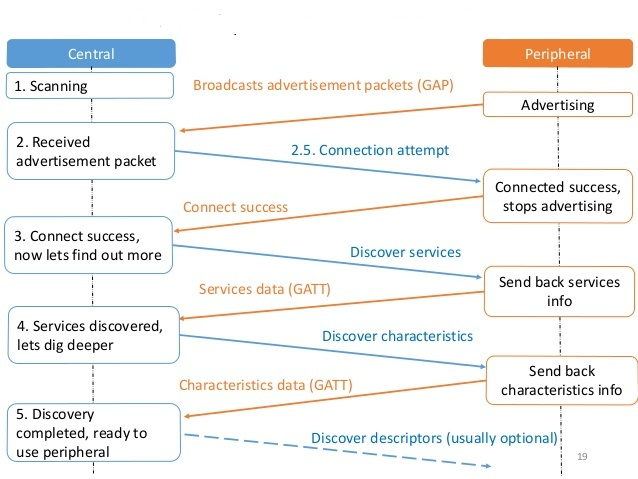
\includegraphics[width=1.0\textwidth]{btwork}
		\caption[Sơ đồ hoạt động của BLE]{Sơ đồ hoạt động của BLE}
		\label{fig: btwork}
	\end{figure}
	
\newpage
\subsection{Các vi điều khiển tích hợp công nghệ BLE}
%TODO : ref http://www.argenox.com/bluetooth-low-energy-ble-v4-0-development/library/a-guide-to-selecting-a-bluetooth-chipset/
Các SoC tích hợp sẵn công nghệ BLE phố biến có thể kể đến:

• Texas Instruments: CC2540/CC2541, dòng CC256x, CC26xx

• Nordic Semiconductor: nRF51822, nRF8001

• CSR CSR101x

• Cypress Semiconductor PSoC 4 BLE / PRoC BLE

Tuy nhiên ở Việt Nam tại thời điểm bắt đầu nghiên cứu và hiện thực đề tài thì 2 loại chipset phổ biến và có giá tiền phổ thông là CC2540 và CC2541 được cung cấp theo dạng Module HM-10.
	\begin{figure}[h]
		\centering    
		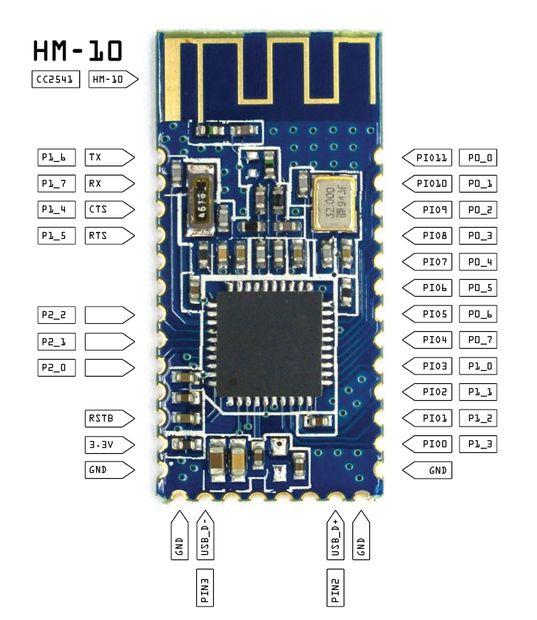
\includegraphics[width=0.4\textwidth]{hm10}
		\caption[Module HM-10]{Module HM-10}
		\label{fig: hm10}
	\end{figure}



\nomenclature[z-FEM]{FEM}{Finite Element Method}
\nomenclature[z-PFEM]{PFEM}{Particle Finite Element Method}
\nomenclature[z-FVM]{FVM}{Finite Volume Method}
\nomenclature[z-BEM]{BEM}{Boundary Element Method}
\nomenclature[z-MPM]{MPM}{Material Point Method}
\nomenclature[z-LBM]{LBM}{Lattice Boltzmann Method}
\nomenclature[z-MRT]{MRT}{Multi-Relaxation 
Time}
\nomenclature[z-RVE]{RVE}{Representative Elemental Volume}
\nomenclature[z-GPU]{GPU}{Graphics Processing Unit}
\nomenclature[z-SH]{SH}{Savage Hutter}
\nomenclature[z-CFD]{CFD}{Computational Fluid Dynamics}
\nomenclature[z-LES]{LES}{Large Eddy Simulation}
\nomenclature[z-FLOP]{FLOP}{Floating Point Operations}
\nomenclature[z-ALU]{ALU}{Arithmetic Logic Unit}
\nomenclature[z-FPU]{FPU}{Floating Point Unit}
\nomenclature[z-SM]{SM}{Streaming Multiprocessors}
\nomenclature[z-PCI]{PCI}{Peripheral Component Interconnect}
\nomenclature[z-CK]{CK}{Carman - Kozeny}
\nomenclature[z-CD]{CD}{Contact Dynamics}
\nomenclature[z-DNS]{DNS}{Direct Numerical Simulation}
\nomenclature[z-EFG]{EFG}{Element-Free Galerkin}
\nomenclature[z-PIC]{PIC}{Particle-in-cell}
\nomenclature[z-USF]{USF}{Update Stress First}
\nomenclature[z-USL]{USL}{Update Stress Last}
\nomenclature[s-crit]{crit}{Critical state}
\nomenclature[z-DKT]{DKT}{Draft Kiss Tumble}
\nomenclature[z-PPC]{PPC}{Particles per cell}